\documentclass[english,letterpaper,11pt]{article}
\usepackage[variablett]{lmodern}	
\usepackage[T1]{fontenc}
\usepackage[utf8]{inputenc}
\usepackage{babel}
\usepackage[babel=true]{microtype}
\usepackage[defaultlines=4,all]{nowidow}
\usepackage{float}
\usepackage[headheight=27pt,margin=1in]{geometry}
\usepackage{parskip}
\usepackage{graphicx}
\usepackage{tikz}
\usepackage{ctable}
\usepackage{csquotes}
\usepackage{fancyhdr}
\usepackage{siunitx} \sisetup{detect-all} %Use with ss fonts
\usepackage[colorlinks, allcolors=black, urlcolor=blue]{hyperref}

\newcommand{\name}{2020 Remote Robot Challenge}
\newcommand{\desc}{Competition Handbook}
\newcommand{\rev}{0}
\newcommand{\registration}{February 28, 2020}
\newcommand{\documentation}{March 27, 2020}
\newcommand{\network}{April 10, 2020}
\newcommand{\los}{April 24, 2020}
\newcommand{\competition}{April 25, 2020}

\newcommand{\CT}[1]{{\color{blue}#1}}
\newcommand{\FC}[1]{{\color{red}#1}}


\renewcommand{\familydefault}{\sfdefault}

\pagestyle{fancy}
\lhead{\scalebox{.15}{
\definecolor{cd95900}{RGB}{217,89,0}

\begin{tikzpicture}[y=0.80pt, x=0.80pt, yscale=-1.000000, xscale=1.000000, inner sep=0pt, outer sep=0pt]
  \begin{scope}[shift={(757.04133,-334.16673)}]
      \path[fill=black] (264.5938,637.6875) .. controls (246.7812,637.9174) and
        (229.3836,672.1698) .. (228.5312,707.0625) .. controls (228.5639,709.8405) and
        (228.6607,712.4932) .. (228.7812,715.0938) -- (252.8125,715.0938) .. controls
        (252.6678,713.4180) and (252.5624,711.6945) .. (252.4688,709.9375) .. controls
        (252.4737,668.5058) and (267.8920,638.6056) .. (293.6250,681.2188) .. controls
        (286.1214,649.6455) and (275.2812,637.5495) .. (264.5938,637.6875) -- cycle;
      \path[fill=black] (401.5850,658.1569) .. controls (402.3485,723.1627) and
        (446.3957,702.3474) .. (439.3173,658.1569) .. controls (434.4405,700.8983) and
        (416.9892,692.3051) .. (415.2562,659.7967) .. controls (415.2592,636.1269) and
        (424.0693,619.0544) .. (438.7705,643.3991) .. controls (427.3390,595.2986) and
        (402.3642,626.2624) .. (401.5850,658.1569) -- cycle;
      \path[fill=black] (325.4857,656.0686) .. controls (326.3531,730.1776) and
        (376.3942,706.4474) .. (368.3526,656.0686) .. controls (362.8121,704.7953) and
        (342.9861,694.9988) .. (341.0172,657.9379) .. controls (341.0202,630.9535) and
        (351.0297,611.4902) .. (367.7313,639.2441) .. controls (354.7442,584.4077) and
        (326.3709,619.7076) .. (325.4857,656.0686) -- cycle;
      \path[fill=black] (345.8342,725.4132) -- (267.5344,706.8995) --
        (355.0955,653.8828) -- (413.1889,659.7736) -- (390.4567,690.0688) --
        (372.7761,672.3966) -- cycle;
      \path[fill=black] (301.6797,700.3034) -- (319.3603,696.9872) .. controls
        (316.7614,638.6511) and (315.6229,599.5835) .. (311.1093,533.2484) .. controls
        (306.9897,593.9198) and (304.6017,651.4817) .. (301.6797,700.3034) -- cycle;
    \path[fill=black] (326.3817,541.1868) .. controls (326.3817,549.4685) and
      (319.6649,556.1822) .. (311.3792,556.1822) .. controls (303.0936,556.1822) and
      (296.3768,549.4685) .. (296.3768,541.1868) .. controls (296.3768,532.9051) and
      (303.0936,526.1914) .. (311.3792,526.1914) .. controls (319.6649,526.1914) and
      (326.3817,532.9051) .. (326.3817,541.1868) -- cycle;
  \end{scope}
  \begin{scope}[fill=black]
    \path[fill=black] (866.2387,487.4175) .. controls (866.2387,489.4569) and
      (865.6178,491.1716) .. (864.3759,492.5616) .. controls (863.1341,493.9515) and
      (861.4479,494.9997) .. (859.3173,495.7061) -- (865.1962,506.4556) --
      (857.8647,506.4556) -- (853.0795,497.1245) -- (849.3881,497.1245) --
      (847.2348,506.4556) -- (840.6723,506.4556) -- (846.5512,481.0088) --
      (856.4804,481.0088) .. controls (859.5908,481.0088) and (861.9947,481.5386) ..
      (863.6923,482.5982) .. controls (865.3899,483.6464) and (866.2387,485.2528) ..
      (866.2387,487.4175) -- cycle(859.1635,488.5113) .. controls
      (859.1635,487.4859) and (858.8331,486.7624) .. (858.1723,486.3408) .. controls
      (857.5229,485.9079) and (856.5602,485.6914) .. (855.2841,485.6914) --
      (852.0370,485.6914) -- (850.4477,492.5445) -- (853.6777,492.5445) .. controls
      (855.4208,492.5445) and (856.7709,492.1913) .. (857.7280,491.4849) .. controls
      (858.6850,490.7671) and (859.1635,489.7759) .. (859.1635,488.5113) -- cycle;
    \path[fill=black] (892.4033,481.0088) -- (891.2924,485.8282) --
      (879.4150,485.8282) -- (878.3554,490.3741) -- (889.3784,490.3741) --
      (888.2504,495.2105) -- (877.2275,495.2105) -- (875.7407,501.6363) --
      (887.6181,501.6363) -- (886.5244,506.4556) -- (868.0844,506.4556) --
      (873.9633,481.0088) -- cycle;
    \path[fill=black] (918.7216,506.4556) -- (912.1591,506.4556) --
      (916.0043,489.8101) -- (909.0146,500.4742) -- (904.4858,500.4742) --
      (902.2299,489.1094) -- (898.2309,506.4556) -- (892.0102,506.4556) --
      (897.8891,481.0088) -- (905.4257,481.0088) -- (908.2114,493.7749) --
      (916.8588,481.0088) -- (924.6005,481.0088) -- cycle;
    \path[fill=black] (953.3285,490.4766) .. controls (953.3285,492.5615) and
      (952.9754,494.6123) .. (952.2690,496.6289) .. controls (951.5626,498.6455) and
      (950.5372,500.4058) .. (949.1928,501.9097) .. controls (947.7231,503.5503) and
      (946.0084,504.8093) .. (944.0488,505.6866) .. controls (942.0891,506.5524) and
      (939.8333,506.9854) .. (937.2812,506.9854) .. controls (933.8063,506.9854) and
      (931.0833,506.0910) .. (929.1122,504.3023) .. controls (927.1526,502.5021) and
      (926.1728,500.0298) .. (926.1728,496.8853) .. controls (926.1728,494.6750) and
      (926.5488,492.5729) .. (927.3007,490.5791) .. controls (928.0527,488.5853) and
      (929.1293,486.8308) .. (930.5307,485.3155) .. controls (931.8979,483.8457) and
      (933.5898,482.6722) .. (935.6064,481.7950) .. controls (937.6230,480.9177) and
      (939.8219,480.4790) .. (942.2031,480.4790) .. controls (945.6894,480.4790) and
      (948.4124,481.3791) .. (950.3720,483.1792) .. controls (952.3430,484.9794) and
      (953.3285,487.4118) .. (953.3285,490.4766) -- cycle(943.9462,499.1582) ..
      controls (944.7210,498.1442) and (945.3248,496.9707) .. (945.7577,495.6377) ..
      controls (946.2021,494.2933) and (946.4243,492.7495) .. (946.4243,491.0064) ..
      controls (946.4243,489.1835) and (945.9856,487.7593) .. (945.1083,486.7339) ..
      controls (944.2425,485.6971) and (943.0006,485.1787) .. (941.3827,485.1787) ..
      controls (940.3232,485.1787) and (939.3092,485.4237) .. (938.3408,485.9136) ..
      controls (937.3837,486.3921) and (936.5007,487.1270) .. (935.6918,488.1182) ..
      controls (934.9057,489.0638) and (934.2734,490.2430) .. (933.7949,491.6558) ..
      controls (933.3163,493.0572) and (933.0771,494.6351) .. (933.0771,496.3897) ..
      controls (933.0771,498.3379) and (933.5214,499.8076) .. (934.4101,500.7989) ..
      controls (935.3102,501.7901) and (936.5520,502.2857) .. (938.1357,502.2857) ..
      controls (939.2294,502.2857) and (940.2833,502.0179) .. (941.2973,501.4824) ..
      controls (942.3113,500.9356) and (943.1943,500.1608) .. (943.9462,499.1582) --
      cycle;
    \path[fill=black] (979.5956,485.9307) -- (971.6659,485.9307) --
      (966.9321,506.4556) -- (960.3354,506.4556) -- (965.0693,485.9307) --
      (957.1396,485.9307) -- (958.2675,481.0088) -- (980.7236,481.0088) -- cycle;
    \path[fill=black] (1003.0771,481.0088) -- (1001.9662,485.8282) --
      (990.0888,485.8282) -- (989.0292,490.3741) -- (1000.0522,490.3741) --
      (998.9243,495.2105) -- (987.9013,495.2105) -- (986.4145,501.6363) --
      (998.2919,501.6363) -- (997.1982,506.4556) -- (978.7582,506.4556) --
      (984.6372,481.0088) -- cycle;
    \path[fill=black] (1040.2133,487.4175) .. controls (1040.2133,489.4569) and
      (1039.5924,491.1716) .. (1038.3505,492.5616) .. controls (1037.1086,493.9515)
      and (1035.4224,494.9997) .. (1033.2919,495.7061) -- (1039.1708,506.4556) --
      (1031.8393,506.4556) -- (1027.0541,497.1245) -- (1023.3627,497.1245) --
      (1021.2094,506.4556) -- (1014.6469,506.4556) -- (1020.5258,481.0088) --
      (1030.4550,481.0088) .. controls (1033.5653,481.0088) and (1035.9693,481.5386)
      .. (1037.6669,482.5982) .. controls (1039.3645,483.6464) and
      (1040.2133,485.2528) .. (1040.2133,487.4175) -- cycle(1033.1381,488.5113) ..
      controls (1033.1381,487.4859) and (1032.8077,486.7624) .. (1032.1469,486.3408)
      .. controls (1031.4975,485.9079) and (1030.5348,485.6914) ..
      (1029.2587,485.6914) -- (1026.0117,485.6914) -- (1024.4223,492.5445) --
      (1027.6523,492.5445) .. controls (1029.3954,492.5445) and (1030.7455,492.1913)
      .. (1031.7026,491.4849) .. controls (1032.6596,490.7671) and
      (1033.1381,489.7759) .. (1033.1381,488.5113) -- cycle;
    \path[fill=black] (1070.2231,490.4766) .. controls (1070.2231,492.5615) and
      (1069.8699,494.6123) .. (1069.1635,496.6289) .. controls (1068.4571,498.6455)
      and (1067.4317,500.4058) .. (1066.0873,501.9097) .. controls
      (1064.6176,503.5503) and (1062.9030,504.8093) .. (1060.9433,505.6866) ..
      controls (1058.9836,506.5524) and (1056.7278,506.9854) .. (1054.1757,506.9854)
      .. controls (1050.7008,506.9854) and (1047.9778,506.0910) ..
      (1046.0068,504.3023) .. controls (1044.0471,502.5021) and (1043.0673,500.0298)
      .. (1043.0673,496.8853) .. controls (1043.0673,494.6750) and
      (1043.4433,492.5729) .. (1044.1953,490.5791) .. controls (1044.9472,488.5853)
      and (1046.0239,486.8308) .. (1047.4252,485.3155) .. controls
      (1048.7924,483.8457) and (1050.4843,482.6722) .. (1052.5009,481.7950) ..
      controls (1054.5175,480.9177) and (1056.7164,480.4790) .. (1059.0976,480.4790)
      .. controls (1062.5839,480.4790) and (1065.3069,481.3791) ..
      (1067.2665,483.1792) .. controls (1069.2376,484.9794) and (1070.2231,487.4118)
      .. (1070.2231,490.4766) -- cycle(1060.8408,499.1582) .. controls
      (1061.6155,498.1442) and (1062.2194,496.9707) .. (1062.6523,495.6377) ..
      controls (1063.0966,494.2933) and (1063.3188,492.7495) .. (1063.3188,491.0064)
      .. controls (1063.3188,489.1835) and (1062.8802,487.7593) ..
      (1062.0029,486.7339) .. controls (1061.1370,485.6971) and (1059.8951,485.1787)
      .. (1058.2773,485.1787) .. controls (1057.2177,485.1787) and
      (1056.2037,485.4237) .. (1055.2353,485.9136) .. controls (1054.2782,486.3921)
      and (1053.3953,487.1270) .. (1052.5864,488.1182) .. controls
      (1051.8003,489.0638) and (1051.1679,490.2430) .. (1050.6894,491.6558) ..
      controls (1050.2109,493.0572) and (1049.9716,494.6351) .. (1049.9716,496.3897)
      .. controls (1049.9716,498.3379) and (1050.4159,499.8076) ..
      (1051.3046,500.7989) .. controls (1052.2047,501.7901) and (1053.4465,502.2857)
      .. (1055.0302,502.2857) .. controls (1056.1239,502.2857) and
      (1057.1778,502.0179) .. (1058.1918,501.4824) .. controls (1059.2058,500.9356)
      and (1060.0888,500.1608) .. (1060.8408,499.1582) -- cycle;
    \path[fill=black] (1096.4047,486.7681) .. controls (1096.4047,488.3176) and
      (1095.9775,489.5993) .. (1095.1230,490.6133) .. controls (1094.2799,491.6159)
      and (1092.9867,492.3736) .. (1091.2436,492.8863) -- (1091.2096,493.0230) ..
      controls (1092.5882,493.4217) and (1093.6307,493.9971) .. (1094.3371,494.7491)
      .. controls (1095.0548,495.5010) and (1095.4137,496.5606) ..
      (1095.4137,497.9278) .. controls (1095.4137,500.6052) and (1094.3143,502.6958)
      .. (1092.1154,504.1997) .. controls (1089.9279,505.7036) and
      (1086.8289,506.4556) .. (1082.8185,506.4556) -- (1071.7955,506.4556) --
      (1077.6745,481.0088) -- (1086.9542,481.0088) .. controls (1090.0190,481.0088)
      and (1092.3603,481.5158) .. (1093.9782,482.5298) .. controls
      (1095.5960,483.5324) and (1096.4049,484.9452) .. (1096.4049,486.7681) --
      cycle(1089.4662,487.8106) .. controls (1089.4662,487.0586) and
      (1089.1700,486.5174) .. (1088.5776,486.1870) .. controls (1087.9851,485.8452)
      and (1087.1648,485.6744) .. (1086.1166,485.6744) -- (1083.1601,485.6744) --
      (1081.9125,491.0577) -- (1084.9033,491.0577) .. controls (1086.3388,491.0577)
      and (1087.4554,490.7842) .. (1088.2529,490.2373) .. controls
      (1089.0618,489.6791) and (1089.4662,488.8701) .. (1089.4662,487.8106) --
      cycle(1088.7314,498.0987) .. controls (1088.7314,497.1644) and
      (1088.3782,496.4922) .. (1087.6718,496.0821) .. controls (1086.9654,495.6605)
      and (1085.8546,495.4497) .. (1084.3393,495.4497) -- (1080.9042,495.4497) --
      (1079.4345,501.7901) -- (1082.7499,501.7901) .. controls (1084.6640,501.7901)
      and (1086.1394,501.4768) .. (1087.1762,500.8501) .. controls
      (1088.2130,500.2235) and (1088.7314,499.3063) .. (1088.7314,498.0987) --
      cycle;
    \path[fill=black] (1126.6196,490.4766) .. controls (1126.6196,492.5615) and
      (1126.2664,494.6123) .. (1125.5600,496.6289) .. controls (1124.8536,498.6455)
      and (1123.8282,500.4058) .. (1122.4838,501.9097) .. controls
      (1121.0141,503.5503) and (1119.2994,504.8093) .. (1117.3398,505.6866) ..
      controls (1115.3801,506.5524) and (1113.1243,506.9854) .. (1110.5722,506.9854)
      .. controls (1107.0973,506.9854) and (1104.3743,506.0910) ..
      (1102.4033,504.3023) .. controls (1100.4436,502.5021) and (1099.4638,500.0298)
      .. (1099.4638,496.8853) .. controls (1099.4638,494.6750) and
      (1099.8398,492.5729) .. (1100.5917,490.5791) .. controls (1101.3437,488.5853)
      and (1102.4204,486.8308) .. (1103.8217,485.3155) .. controls
      (1105.1889,483.8457) and (1106.8808,482.6722) .. (1108.8974,481.7950) ..
      controls (1110.9140,480.9177) and (1113.1129,480.4790) .. (1115.4941,480.4790)
      .. controls (1118.9804,480.4790) and (1121.7034,481.3791) ..
      (1123.6630,483.1792) .. controls (1125.6341,484.9794) and (1126.6196,487.4118)
      .. (1126.6196,490.4766) -- cycle(1117.2372,499.1582) .. controls
      (1118.0120,498.1442) and (1118.6159,496.9707) .. (1119.0488,495.6377) ..
      controls (1119.4931,494.2933) and (1119.7153,492.7495) .. (1119.7153,491.0064)
      .. controls (1119.7153,489.1835) and (1119.2767,487.7593) ..
      (1118.3994,486.7339) .. controls (1117.5335,485.6971) and (1116.2916,485.1787)
      .. (1114.6738,485.1787) .. controls (1113.6142,485.1787) and
      (1112.6002,485.4237) .. (1111.6318,485.9136) .. controls (1110.6747,486.3921)
      and (1109.7917,487.1270) .. (1108.9828,488.1182) .. controls
      (1108.1967,489.0638) and (1107.5644,490.2430) .. (1107.0859,491.6558) ..
      controls (1106.6074,493.0572) and (1106.3681,494.6351) .. (1106.3681,496.3897)
      .. controls (1106.3681,498.3379) and (1106.8124,499.8076) ..
      (1107.7011,500.7989) .. controls (1108.6012,501.7901) and (1109.8430,502.2857)
      .. (1111.4267,502.2857) .. controls (1112.5204,502.2857) and
      (1113.5743,502.0179) .. (1114.5883,501.4824) .. controls (1115.6023,500.9356)
      and (1116.4853,500.1608) .. (1117.2372,499.1582) -- cycle;
    \path[fill=black] (1152.8867,485.9307) -- (1144.9570,485.9307) --
      (1140.2231,506.4556) -- (1133.6264,506.4556) -- (1138.3603,485.9307) --
      (1130.4306,485.9307) -- (1131.5585,481.0088) -- (1154.0146,481.0088) -- cycle;
    \path[fill=black] (1175.7870,506.9512) .. controls (1172.3463,506.9512) and
      (1169.6917,506.1081) .. (1167.8232,504.4219) .. controls (1165.9547,502.7243)
      and (1165.0204,500.2976) .. (1165.0204,497.1416) .. controls
      (1165.0204,494.6465) and (1165.4306,492.3850) .. (1166.2509,490.3570) ..
      controls (1167.0826,488.3290) and (1168.2220,486.5744) .. (1169.6689,485.0933)
      .. controls (1171.0816,483.6577) and (1172.7735,482.5355) ..
      (1174.7446,481.7266) .. controls (1176.7270,480.9177) and (1178.8063,480.5132)
      .. (1180.9824,480.5132) .. controls (1182.7369,480.5132) and
      (1184.3662,480.6955) .. (1185.8701,481.0601) .. controls (1187.3740,481.4133)
      and (1188.7297,481.9374) .. (1189.9374,482.6323) -- (1188.4335,488.8018) --
      (1187.6816,488.8018) .. controls (1186.5992,487.6397) and (1185.5225,486.7852)
      .. (1184.4516,486.2383) .. controls (1183.3807,485.6914) and
      (1182.1217,485.4180) .. (1180.6747,485.4180) .. controls (1178.1340,485.4180)
      and (1176.0377,486.4377) .. (1174.3857,488.4771) .. controls
      (1172.7450,490.5165) and (1171.9247,493.1141) .. (1171.9247,496.2700) ..
      controls (1171.9247,498.2980) and (1172.3804,499.7678) .. (1173.2919,500.6792)
      .. controls (1174.2034,501.5907) and (1175.5364,502.0464) ..
      (1177.2910,502.0464) .. controls (1178.8633,502.0464) and (1180.3387,501.7331)
      .. (1181.7172,501.1065) .. controls (1183.0958,500.4685) and
      (1184.4003,499.6595) .. (1185.6308,498.6797) -- (1186.3144,498.6797) --
      (1184.8276,504.7637) .. controls (1184.3149,504.9688) and (1183.7167,505.2194)
      .. (1183.0331,505.5157) .. controls (1182.3496,505.8005) and
      (1181.6945,506.0340) .. (1181.0678,506.2163) .. controls (1180.2475,506.4556)
      and (1179.4784,506.6379) .. (1178.7607,506.7632) .. controls
      (1178.0543,506.8885) and (1177.0631,506.9512) .. (1175.7870,506.9512) --
      cycle;
    \path[fill=black] (1218.1015,481.0088) -- (1212.2226,506.4556) --
      (1205.6259,506.4556) -- (1208.2236,495.2105) -- (1198.5678,495.2105) --
      (1195.9702,506.4556) -- (1189.3735,506.4556) -- (1195.2524,481.0088) --
      (1201.8491,481.0088) -- (1199.6786,490.3741) -- (1209.3344,490.3741) --
      (1211.5048,481.0088) -- cycle;
    \path[fill=black] (1242.4887,506.4556) -- (1235.8749,506.4556) --
      (1235.2939,501.2603) -- (1225.9286,501.2603) -- (1222.9550,506.4556) --
      (1216.1020,506.4556) -- (1231.3632,481.0088) -- (1238.9511,481.0088) --
      cycle(1234.7983,496.6973) -- (1233.7729,487.5542) -- (1228.5263,496.6973) --
      cycle;
    \path[fill=black] (1264.2783,506.4556) -- (1245.9067,506.4556) --
      (1251.7856,481.0088) -- (1258.3823,481.0088) -- (1253.6484,501.5337) --
      (1265.4233,501.5337) -- cycle;
    \path[fill=black] (1286.5634,506.4556) -- (1268.1918,506.4556) --
      (1274.0707,481.0088) -- (1280.6674,481.0088) -- (1275.9335,501.5337) --
      (1287.7084,501.5337) -- cycle;
    \path[fill=black] (1314.7958,481.0088) -- (1313.6850,485.8282) --
      (1301.8076,485.8282) -- (1300.7480,490.3741) -- (1311.7709,490.3741) --
      (1310.6430,495.2105) -- (1299.6201,495.2105) -- (1298.1332,501.6363) --
      (1310.0107,501.6363) -- (1308.9169,506.4556) -- (1290.4770,506.4556) --
      (1296.3559,481.0088) -- cycle;
    \path[fill=black] (1337.5766,506.4556) -- (1331.9882,506.4556) --
      (1324.5200,488.8360) -- (1320.4526,506.4556) -- (1314.4028,506.4556) --
      (1320.2817,481.0088) -- (1327.6303,481.0088) -- (1334.0219,495.7403) --
      (1337.4057,481.0088) -- (1343.4555,481.0088) -- cycle;
    \path[fill=black] (1356.6318,506.9854) .. controls (1353.0201,506.9854) and
      (1350.1889,506.1309) .. (1348.1381,504.4219) .. controls (1346.0987,502.7129)
      and (1345.0790,500.2862) .. (1345.0790,497.1416) .. controls
      (1345.0790,492.2425) and (1346.6570,488.2492) .. (1349.8129,485.1617) ..
      controls (1352.9688,482.0627) and (1356.9736,480.5132) .. (1361.8271,480.5132)
      .. controls (1363.6614,480.5132) and (1365.3590,480.6727) ..
      (1366.9199,480.9917) .. controls (1368.4922,481.2994) and (1370.1214,481.8918)
      .. (1371.8076,482.7691) -- (1370.3549,488.7334) -- (1369.6201,488.7334) ..
      controls (1368.2529,487.4346) and (1366.9598,486.5345) .. (1365.7407,486.0332)
      .. controls (1364.5216,485.5205) and (1363.1772,485.2642) ..
      (1361.7075,485.2642) .. controls (1360.2150,485.2642) and (1358.8649,485.5718)
      .. (1357.6572,486.1870) .. controls (1356.4495,486.7909) and
      (1355.4184,487.6112) .. (1354.5639,488.6480) .. controls (1353.7550,489.6278)
      and (1353.1226,490.7899) .. (1352.6669,492.1343) .. controls
      (1352.2112,493.4787) and (1351.9833,494.8858) .. (1351.9833,496.3555) ..
      controls (1351.9833,498.3949) and (1352.5416,499.8988) .. (1353.6581,500.8672)
      .. controls (1354.7746,501.8242) and (1356.5919,502.3028) ..
      (1359.1098,502.3028) .. controls (1359.3605,502.3028) and (1359.6339,502.2971)
      .. (1359.9301,502.2857) .. controls (1360.2264,502.2743) and
      (1360.4998,502.2572) .. (1360.7504,502.2344) -- (1361.9125,497.2441) --
      (1356.8369,497.2441) -- (1357.9477,492.4419) -- (1369.6884,492.4419) --
      (1366.7831,505.0029) .. controls (1365.2678,505.5270) and (1363.6500,505.9884)
      .. (1361.9296,506.3872) .. controls (1360.2206,506.7859) and
      (1358.4547,506.9853) .. (1356.6318,506.9853) -- cycle;
    \path[fill=black] (1396.7587,481.0088) -- (1395.6479,485.8282) --
      (1383.7704,485.8282) -- (1382.7109,490.3741) -- (1393.7338,490.3741) --
      (1392.6059,495.2105) -- (1381.5829,495.2105) -- (1380.0961,501.6363) --
      (1391.9736,501.6363) -- (1390.8798,506.4556) -- (1372.4399,506.4556) --
      (1378.3188,481.0088) -- cycle;
  \end{scope}
  \begin{scope}[shift={(748.4699,-164.16673)}]
    \path[fill=cd95900] (340.9304,561.5005) .. controls (342.2667,675.2871) and
      (419.3673,638.8519) .. (406.9772,561.5005) .. controls (398.4407,636.3153) and
      (367.8939,621.2737) .. (364.8603,564.3707) .. controls (364.8653,522.9391) and
      (380.2870,493.0552) .. (406.0200,535.6683) .. controls (386.0102,451.4729) and
      (342.2941,505.6721) .. (340.9304,561.5005) -- cycle;
    \begin{scope}[shift={(18.61506,-2.36127)},fill=cd95900]
      \path[fill=cd95900] (176.2612,635.3184) -- (154.8873,635.3184) --
        (148.8063,587.9947) -- (128.9375,635.3184) -- (120.4482,635.3184) --
        (101.4826,587.9947) -- (94.4984,635.3184) -- (73.2449,635.3184) --
        (87.2132,553.1341) -- (108.2861,553.1341) -- (124.9638,596.9657) --
        (142.6048,553.1341) -- (163.8583,553.1341) -- cycle;
      \path[fill=cd95900] (236.6501,635.3184) -- (189.8683,635.3184) --
        (189.8683,553.1341) -- (236.6501,553.1341) -- (236.6501,571.0159) --
        (211.2422,571.0159) -- (211.2422,584.9240) -- (235.2653,584.9240) --
        (235.2653,602.8059) -- (211.2422,602.8059) -- (211.2422,617.4365) --
        (236.6501,617.4365) -- cycle;
      \path[fill=cd95900] (318.6538,635.3184) -- (292.0417,635.3184) --
        (271.6913,603.7692) -- (271.6913,635.3184) -- (250.3174,635.3184) --
        (250.3174,553.1341) -- (283.5524,553.1341) .. controls (293.2659,553.1341) and
        (300.4508,556.0442) .. (305.1069,561.8643) .. controls (308.8799,566.5606) and
        (310.7664,572.0797) .. (310.7665,578.4215) .. controls (310.7664,585.6867) and
        (308.5989,591.4868) .. (304.2640,595.8217) .. controls (301.4944,598.5913) and
        (297.6812,600.5180) .. (292.8244,601.6017) -- cycle(288.5497,579.6257) ..
        controls (288.5496,576.6956) and (287.4859,574.2271) .. (285.3586,572.2201) ..
        controls (283.3516,570.3336) and (280.1205,569.3904) .. (275.6651,569.3903) --
        (271.6913,569.3903) -- (271.6913,589.9213) -- (275.6651,589.9213) .. controls
        (280.1606,589.9214) and (283.3918,588.9781) .. (285.3586,587.0915) .. controls
        (287.4859,585.0445) and (288.5496,582.5559) .. (288.5497,579.6257) -- cycle;
      \path[fill=cd95900] (472.0645,600.5180) .. controls (472.0644,605.4551) and
        (471.6630,609.6697) .. (470.8603,613.1617) .. controls (469.6159,618.5805) and
        (466.6457,623.5175) .. (461.9495,627.9729) .. controls (455.2864,634.2747) and
        (446.3756,637.4257) .. (435.2170,637.4257) .. controls (423.8577,637.4257) and
        (414.9870,634.2145) .. (408.6050,627.7923) .. controls (405.2333,624.4207) and
        (402.9253,620.1860) .. (401.6810,615.0884) .. controls (400.7979,611.4759) and
        (400.3564,606.6191) .. (400.3564,600.5180) -- (400.3564,553.1341) --
        (421.7304,553.1341) -- (421.7304,597.6280) .. controls (421.7303,601.2004) and
        (421.7906,603.8696) .. (421.9110,605.6357) .. controls (422.3124,611.2150) and
        (424.8612,615.1085) .. (429.5574,617.3161) .. controls (431.4841,618.2393) and
        (433.6114,618.7009) .. (435.9395,618.7009) .. controls (441.1575,618.7009) and
        (445.0911,616.8746) .. (447.7403,613.2219) .. controls (449.7071,610.5327) and
        (450.6905,605.3347) .. (450.6905,597.6280) -- (450.6905,553.1341) --
        (472.0645,553.1341) -- cycle;
      \path[fill=cd95900] (557.5602,635.3184) -- (530.9482,635.3184) --
        (510.5978,603.7692) -- (510.5978,635.3184) -- (489.2238,635.3184) --
        (489.2238,553.1341) -- (522.4588,553.1341) .. controls (532.1723,553.1341) and
        (539.3572,556.0442) .. (544.0133,561.8643) .. controls (547.7863,566.5606) and
        (549.6729,572.0797) .. (549.6729,578.4215) .. controls (549.6729,585.6867) and
        (547.5054,591.4868) .. (543.1704,595.8217) .. controls (540.4008,598.5913) and
        (536.5876,600.5180) .. (531.7309,601.6017) -- cycle(527.4561,579.6257) ..
        controls (527.4560,576.6956) and (526.3923,574.2271) .. (524.2650,572.2201) ..
        controls (522.2581,570.3336) and (519.0269,569.3904) .. (514.5715,569.3903) --
        (510.5978,569.3903) -- (510.5978,589.9213) -- (514.5715,589.9213) .. controls
        (519.0670,589.9214) and (522.2982,588.9781) .. (524.2650,587.0915) .. controls
        (526.3923,585.0445) and (527.4560,582.5559) .. (527.4561,579.6257) -- cycle;
      \path[fill=cd95900] (638.2995,553.1341) -- (607.5331,595.8217) --
        (607.5331,635.3184) -- (586.1591,635.3184) -- (586.1591,595.8217) --
        (556.4162,553.1341) -- (581.9446,553.1341) -- (597.4783,575.5315) --
        (612.4099,553.1341) -- cycle;
    \end{scope}
  \end{scope}

\end{tikzpicture}}}
\rhead{2020 Competition Handbook \\ Revision \rev}
\cfoot{\thepage}

\begin{document}

\begin{titlepage}
	\centering
	\scalebox{.75}{
\definecolor{cd95900}{RGB}{217,89,0}

\begin{tikzpicture}[y=0.80pt, x=0.80pt, yscale=-1.000000, xscale=1.000000, inner sep=0pt, outer sep=0pt]
  \begin{scope}[shift={(757.04133,-334.16673)}]
      \path[fill=black] (264.5938,637.6875) .. controls (246.7812,637.9174) and
        (229.3836,672.1698) .. (228.5312,707.0625) .. controls (228.5639,709.8405) and
        (228.6607,712.4932) .. (228.7812,715.0938) -- (252.8125,715.0938) .. controls
        (252.6678,713.4180) and (252.5624,711.6945) .. (252.4688,709.9375) .. controls
        (252.4737,668.5058) and (267.8920,638.6056) .. (293.6250,681.2188) .. controls
        (286.1214,649.6455) and (275.2812,637.5495) .. (264.5938,637.6875) -- cycle;
      \path[fill=black] (401.5850,658.1569) .. controls (402.3485,723.1627) and
        (446.3957,702.3474) .. (439.3173,658.1569) .. controls (434.4405,700.8983) and
        (416.9892,692.3051) .. (415.2562,659.7967) .. controls (415.2592,636.1269) and
        (424.0693,619.0544) .. (438.7705,643.3991) .. controls (427.3390,595.2986) and
        (402.3642,626.2624) .. (401.5850,658.1569) -- cycle;
      \path[fill=black] (325.4857,656.0686) .. controls (326.3531,730.1776) and
        (376.3942,706.4474) .. (368.3526,656.0686) .. controls (362.8121,704.7953) and
        (342.9861,694.9988) .. (341.0172,657.9379) .. controls (341.0202,630.9535) and
        (351.0297,611.4902) .. (367.7313,639.2441) .. controls (354.7442,584.4077) and
        (326.3709,619.7076) .. (325.4857,656.0686) -- cycle;
      \path[fill=black] (345.8342,725.4132) -- (267.5344,706.8995) --
        (355.0955,653.8828) -- (413.1889,659.7736) -- (390.4567,690.0688) --
        (372.7761,672.3966) -- cycle;
      \path[fill=black] (301.6797,700.3034) -- (319.3603,696.9872) .. controls
        (316.7614,638.6511) and (315.6229,599.5835) .. (311.1093,533.2484) .. controls
        (306.9897,593.9198) and (304.6017,651.4817) .. (301.6797,700.3034) -- cycle;
    \path[fill=black] (326.3817,541.1868) .. controls (326.3817,549.4685) and
      (319.6649,556.1822) .. (311.3792,556.1822) .. controls (303.0936,556.1822) and
      (296.3768,549.4685) .. (296.3768,541.1868) .. controls (296.3768,532.9051) and
      (303.0936,526.1914) .. (311.3792,526.1914) .. controls (319.6649,526.1914) and
      (326.3817,532.9051) .. (326.3817,541.1868) -- cycle;
  \end{scope}
  \begin{scope}[fill=black]
    \path[fill=black] (866.2387,487.4175) .. controls (866.2387,489.4569) and
      (865.6178,491.1716) .. (864.3759,492.5616) .. controls (863.1341,493.9515) and
      (861.4479,494.9997) .. (859.3173,495.7061) -- (865.1962,506.4556) --
      (857.8647,506.4556) -- (853.0795,497.1245) -- (849.3881,497.1245) --
      (847.2348,506.4556) -- (840.6723,506.4556) -- (846.5512,481.0088) --
      (856.4804,481.0088) .. controls (859.5908,481.0088) and (861.9947,481.5386) ..
      (863.6923,482.5982) .. controls (865.3899,483.6464) and (866.2387,485.2528) ..
      (866.2387,487.4175) -- cycle(859.1635,488.5113) .. controls
      (859.1635,487.4859) and (858.8331,486.7624) .. (858.1723,486.3408) .. controls
      (857.5229,485.9079) and (856.5602,485.6914) .. (855.2841,485.6914) --
      (852.0370,485.6914) -- (850.4477,492.5445) -- (853.6777,492.5445) .. controls
      (855.4208,492.5445) and (856.7709,492.1913) .. (857.7280,491.4849) .. controls
      (858.6850,490.7671) and (859.1635,489.7759) .. (859.1635,488.5113) -- cycle;
    \path[fill=black] (892.4033,481.0088) -- (891.2924,485.8282) --
      (879.4150,485.8282) -- (878.3554,490.3741) -- (889.3784,490.3741) --
      (888.2504,495.2105) -- (877.2275,495.2105) -- (875.7407,501.6363) --
      (887.6181,501.6363) -- (886.5244,506.4556) -- (868.0844,506.4556) --
      (873.9633,481.0088) -- cycle;
    \path[fill=black] (918.7216,506.4556) -- (912.1591,506.4556) --
      (916.0043,489.8101) -- (909.0146,500.4742) -- (904.4858,500.4742) --
      (902.2299,489.1094) -- (898.2309,506.4556) -- (892.0102,506.4556) --
      (897.8891,481.0088) -- (905.4257,481.0088) -- (908.2114,493.7749) --
      (916.8588,481.0088) -- (924.6005,481.0088) -- cycle;
    \path[fill=black] (953.3285,490.4766) .. controls (953.3285,492.5615) and
      (952.9754,494.6123) .. (952.2690,496.6289) .. controls (951.5626,498.6455) and
      (950.5372,500.4058) .. (949.1928,501.9097) .. controls (947.7231,503.5503) and
      (946.0084,504.8093) .. (944.0488,505.6866) .. controls (942.0891,506.5524) and
      (939.8333,506.9854) .. (937.2812,506.9854) .. controls (933.8063,506.9854) and
      (931.0833,506.0910) .. (929.1122,504.3023) .. controls (927.1526,502.5021) and
      (926.1728,500.0298) .. (926.1728,496.8853) .. controls (926.1728,494.6750) and
      (926.5488,492.5729) .. (927.3007,490.5791) .. controls (928.0527,488.5853) and
      (929.1293,486.8308) .. (930.5307,485.3155) .. controls (931.8979,483.8457) and
      (933.5898,482.6722) .. (935.6064,481.7950) .. controls (937.6230,480.9177) and
      (939.8219,480.4790) .. (942.2031,480.4790) .. controls (945.6894,480.4790) and
      (948.4124,481.3791) .. (950.3720,483.1792) .. controls (952.3430,484.9794) and
      (953.3285,487.4118) .. (953.3285,490.4766) -- cycle(943.9462,499.1582) ..
      controls (944.7210,498.1442) and (945.3248,496.9707) .. (945.7577,495.6377) ..
      controls (946.2021,494.2933) and (946.4243,492.7495) .. (946.4243,491.0064) ..
      controls (946.4243,489.1835) and (945.9856,487.7593) .. (945.1083,486.7339) ..
      controls (944.2425,485.6971) and (943.0006,485.1787) .. (941.3827,485.1787) ..
      controls (940.3232,485.1787) and (939.3092,485.4237) .. (938.3408,485.9136) ..
      controls (937.3837,486.3921) and (936.5007,487.1270) .. (935.6918,488.1182) ..
      controls (934.9057,489.0638) and (934.2734,490.2430) .. (933.7949,491.6558) ..
      controls (933.3163,493.0572) and (933.0771,494.6351) .. (933.0771,496.3897) ..
      controls (933.0771,498.3379) and (933.5214,499.8076) .. (934.4101,500.7989) ..
      controls (935.3102,501.7901) and (936.5520,502.2857) .. (938.1357,502.2857) ..
      controls (939.2294,502.2857) and (940.2833,502.0179) .. (941.2973,501.4824) ..
      controls (942.3113,500.9356) and (943.1943,500.1608) .. (943.9462,499.1582) --
      cycle;
    \path[fill=black] (979.5956,485.9307) -- (971.6659,485.9307) --
      (966.9321,506.4556) -- (960.3354,506.4556) -- (965.0693,485.9307) --
      (957.1396,485.9307) -- (958.2675,481.0088) -- (980.7236,481.0088) -- cycle;
    \path[fill=black] (1003.0771,481.0088) -- (1001.9662,485.8282) --
      (990.0888,485.8282) -- (989.0292,490.3741) -- (1000.0522,490.3741) --
      (998.9243,495.2105) -- (987.9013,495.2105) -- (986.4145,501.6363) --
      (998.2919,501.6363) -- (997.1982,506.4556) -- (978.7582,506.4556) --
      (984.6372,481.0088) -- cycle;
    \path[fill=black] (1040.2133,487.4175) .. controls (1040.2133,489.4569) and
      (1039.5924,491.1716) .. (1038.3505,492.5616) .. controls (1037.1086,493.9515)
      and (1035.4224,494.9997) .. (1033.2919,495.7061) -- (1039.1708,506.4556) --
      (1031.8393,506.4556) -- (1027.0541,497.1245) -- (1023.3627,497.1245) --
      (1021.2094,506.4556) -- (1014.6469,506.4556) -- (1020.5258,481.0088) --
      (1030.4550,481.0088) .. controls (1033.5653,481.0088) and (1035.9693,481.5386)
      .. (1037.6669,482.5982) .. controls (1039.3645,483.6464) and
      (1040.2133,485.2528) .. (1040.2133,487.4175) -- cycle(1033.1381,488.5113) ..
      controls (1033.1381,487.4859) and (1032.8077,486.7624) .. (1032.1469,486.3408)
      .. controls (1031.4975,485.9079) and (1030.5348,485.6914) ..
      (1029.2587,485.6914) -- (1026.0117,485.6914) -- (1024.4223,492.5445) --
      (1027.6523,492.5445) .. controls (1029.3954,492.5445) and (1030.7455,492.1913)
      .. (1031.7026,491.4849) .. controls (1032.6596,490.7671) and
      (1033.1381,489.7759) .. (1033.1381,488.5113) -- cycle;
    \path[fill=black] (1070.2231,490.4766) .. controls (1070.2231,492.5615) and
      (1069.8699,494.6123) .. (1069.1635,496.6289) .. controls (1068.4571,498.6455)
      and (1067.4317,500.4058) .. (1066.0873,501.9097) .. controls
      (1064.6176,503.5503) and (1062.9030,504.8093) .. (1060.9433,505.6866) ..
      controls (1058.9836,506.5524) and (1056.7278,506.9854) .. (1054.1757,506.9854)
      .. controls (1050.7008,506.9854) and (1047.9778,506.0910) ..
      (1046.0068,504.3023) .. controls (1044.0471,502.5021) and (1043.0673,500.0298)
      .. (1043.0673,496.8853) .. controls (1043.0673,494.6750) and
      (1043.4433,492.5729) .. (1044.1953,490.5791) .. controls (1044.9472,488.5853)
      and (1046.0239,486.8308) .. (1047.4252,485.3155) .. controls
      (1048.7924,483.8457) and (1050.4843,482.6722) .. (1052.5009,481.7950) ..
      controls (1054.5175,480.9177) and (1056.7164,480.4790) .. (1059.0976,480.4790)
      .. controls (1062.5839,480.4790) and (1065.3069,481.3791) ..
      (1067.2665,483.1792) .. controls (1069.2376,484.9794) and (1070.2231,487.4118)
      .. (1070.2231,490.4766) -- cycle(1060.8408,499.1582) .. controls
      (1061.6155,498.1442) and (1062.2194,496.9707) .. (1062.6523,495.6377) ..
      controls (1063.0966,494.2933) and (1063.3188,492.7495) .. (1063.3188,491.0064)
      .. controls (1063.3188,489.1835) and (1062.8802,487.7593) ..
      (1062.0029,486.7339) .. controls (1061.1370,485.6971) and (1059.8951,485.1787)
      .. (1058.2773,485.1787) .. controls (1057.2177,485.1787) and
      (1056.2037,485.4237) .. (1055.2353,485.9136) .. controls (1054.2782,486.3921)
      and (1053.3953,487.1270) .. (1052.5864,488.1182) .. controls
      (1051.8003,489.0638) and (1051.1679,490.2430) .. (1050.6894,491.6558) ..
      controls (1050.2109,493.0572) and (1049.9716,494.6351) .. (1049.9716,496.3897)
      .. controls (1049.9716,498.3379) and (1050.4159,499.8076) ..
      (1051.3046,500.7989) .. controls (1052.2047,501.7901) and (1053.4465,502.2857)
      .. (1055.0302,502.2857) .. controls (1056.1239,502.2857) and
      (1057.1778,502.0179) .. (1058.1918,501.4824) .. controls (1059.2058,500.9356)
      and (1060.0888,500.1608) .. (1060.8408,499.1582) -- cycle;
    \path[fill=black] (1096.4047,486.7681) .. controls (1096.4047,488.3176) and
      (1095.9775,489.5993) .. (1095.1230,490.6133) .. controls (1094.2799,491.6159)
      and (1092.9867,492.3736) .. (1091.2436,492.8863) -- (1091.2096,493.0230) ..
      controls (1092.5882,493.4217) and (1093.6307,493.9971) .. (1094.3371,494.7491)
      .. controls (1095.0548,495.5010) and (1095.4137,496.5606) ..
      (1095.4137,497.9278) .. controls (1095.4137,500.6052) and (1094.3143,502.6958)
      .. (1092.1154,504.1997) .. controls (1089.9279,505.7036) and
      (1086.8289,506.4556) .. (1082.8185,506.4556) -- (1071.7955,506.4556) --
      (1077.6745,481.0088) -- (1086.9542,481.0088) .. controls (1090.0190,481.0088)
      and (1092.3603,481.5158) .. (1093.9782,482.5298) .. controls
      (1095.5960,483.5324) and (1096.4049,484.9452) .. (1096.4049,486.7681) --
      cycle(1089.4662,487.8106) .. controls (1089.4662,487.0586) and
      (1089.1700,486.5174) .. (1088.5776,486.1870) .. controls (1087.9851,485.8452)
      and (1087.1648,485.6744) .. (1086.1166,485.6744) -- (1083.1601,485.6744) --
      (1081.9125,491.0577) -- (1084.9033,491.0577) .. controls (1086.3388,491.0577)
      and (1087.4554,490.7842) .. (1088.2529,490.2373) .. controls
      (1089.0618,489.6791) and (1089.4662,488.8701) .. (1089.4662,487.8106) --
      cycle(1088.7314,498.0987) .. controls (1088.7314,497.1644) and
      (1088.3782,496.4922) .. (1087.6718,496.0821) .. controls (1086.9654,495.6605)
      and (1085.8546,495.4497) .. (1084.3393,495.4497) -- (1080.9042,495.4497) --
      (1079.4345,501.7901) -- (1082.7499,501.7901) .. controls (1084.6640,501.7901)
      and (1086.1394,501.4768) .. (1087.1762,500.8501) .. controls
      (1088.2130,500.2235) and (1088.7314,499.3063) .. (1088.7314,498.0987) --
      cycle;
    \path[fill=black] (1126.6196,490.4766) .. controls (1126.6196,492.5615) and
      (1126.2664,494.6123) .. (1125.5600,496.6289) .. controls (1124.8536,498.6455)
      and (1123.8282,500.4058) .. (1122.4838,501.9097) .. controls
      (1121.0141,503.5503) and (1119.2994,504.8093) .. (1117.3398,505.6866) ..
      controls (1115.3801,506.5524) and (1113.1243,506.9854) .. (1110.5722,506.9854)
      .. controls (1107.0973,506.9854) and (1104.3743,506.0910) ..
      (1102.4033,504.3023) .. controls (1100.4436,502.5021) and (1099.4638,500.0298)
      .. (1099.4638,496.8853) .. controls (1099.4638,494.6750) and
      (1099.8398,492.5729) .. (1100.5917,490.5791) .. controls (1101.3437,488.5853)
      and (1102.4204,486.8308) .. (1103.8217,485.3155) .. controls
      (1105.1889,483.8457) and (1106.8808,482.6722) .. (1108.8974,481.7950) ..
      controls (1110.9140,480.9177) and (1113.1129,480.4790) .. (1115.4941,480.4790)
      .. controls (1118.9804,480.4790) and (1121.7034,481.3791) ..
      (1123.6630,483.1792) .. controls (1125.6341,484.9794) and (1126.6196,487.4118)
      .. (1126.6196,490.4766) -- cycle(1117.2372,499.1582) .. controls
      (1118.0120,498.1442) and (1118.6159,496.9707) .. (1119.0488,495.6377) ..
      controls (1119.4931,494.2933) and (1119.7153,492.7495) .. (1119.7153,491.0064)
      .. controls (1119.7153,489.1835) and (1119.2767,487.7593) ..
      (1118.3994,486.7339) .. controls (1117.5335,485.6971) and (1116.2916,485.1787)
      .. (1114.6738,485.1787) .. controls (1113.6142,485.1787) and
      (1112.6002,485.4237) .. (1111.6318,485.9136) .. controls (1110.6747,486.3921)
      and (1109.7917,487.1270) .. (1108.9828,488.1182) .. controls
      (1108.1967,489.0638) and (1107.5644,490.2430) .. (1107.0859,491.6558) ..
      controls (1106.6074,493.0572) and (1106.3681,494.6351) .. (1106.3681,496.3897)
      .. controls (1106.3681,498.3379) and (1106.8124,499.8076) ..
      (1107.7011,500.7989) .. controls (1108.6012,501.7901) and (1109.8430,502.2857)
      .. (1111.4267,502.2857) .. controls (1112.5204,502.2857) and
      (1113.5743,502.0179) .. (1114.5883,501.4824) .. controls (1115.6023,500.9356)
      and (1116.4853,500.1608) .. (1117.2372,499.1582) -- cycle;
    \path[fill=black] (1152.8867,485.9307) -- (1144.9570,485.9307) --
      (1140.2231,506.4556) -- (1133.6264,506.4556) -- (1138.3603,485.9307) --
      (1130.4306,485.9307) -- (1131.5585,481.0088) -- (1154.0146,481.0088) -- cycle;
    \path[fill=black] (1175.7870,506.9512) .. controls (1172.3463,506.9512) and
      (1169.6917,506.1081) .. (1167.8232,504.4219) .. controls (1165.9547,502.7243)
      and (1165.0204,500.2976) .. (1165.0204,497.1416) .. controls
      (1165.0204,494.6465) and (1165.4306,492.3850) .. (1166.2509,490.3570) ..
      controls (1167.0826,488.3290) and (1168.2220,486.5744) .. (1169.6689,485.0933)
      .. controls (1171.0816,483.6577) and (1172.7735,482.5355) ..
      (1174.7446,481.7266) .. controls (1176.7270,480.9177) and (1178.8063,480.5132)
      .. (1180.9824,480.5132) .. controls (1182.7369,480.5132) and
      (1184.3662,480.6955) .. (1185.8701,481.0601) .. controls (1187.3740,481.4133)
      and (1188.7297,481.9374) .. (1189.9374,482.6323) -- (1188.4335,488.8018) --
      (1187.6816,488.8018) .. controls (1186.5992,487.6397) and (1185.5225,486.7852)
      .. (1184.4516,486.2383) .. controls (1183.3807,485.6914) and
      (1182.1217,485.4180) .. (1180.6747,485.4180) .. controls (1178.1340,485.4180)
      and (1176.0377,486.4377) .. (1174.3857,488.4771) .. controls
      (1172.7450,490.5165) and (1171.9247,493.1141) .. (1171.9247,496.2700) ..
      controls (1171.9247,498.2980) and (1172.3804,499.7678) .. (1173.2919,500.6792)
      .. controls (1174.2034,501.5907) and (1175.5364,502.0464) ..
      (1177.2910,502.0464) .. controls (1178.8633,502.0464) and (1180.3387,501.7331)
      .. (1181.7172,501.1065) .. controls (1183.0958,500.4685) and
      (1184.4003,499.6595) .. (1185.6308,498.6797) -- (1186.3144,498.6797) --
      (1184.8276,504.7637) .. controls (1184.3149,504.9688) and (1183.7167,505.2194)
      .. (1183.0331,505.5157) .. controls (1182.3496,505.8005) and
      (1181.6945,506.0340) .. (1181.0678,506.2163) .. controls (1180.2475,506.4556)
      and (1179.4784,506.6379) .. (1178.7607,506.7632) .. controls
      (1178.0543,506.8885) and (1177.0631,506.9512) .. (1175.7870,506.9512) --
      cycle;
    \path[fill=black] (1218.1015,481.0088) -- (1212.2226,506.4556) --
      (1205.6259,506.4556) -- (1208.2236,495.2105) -- (1198.5678,495.2105) --
      (1195.9702,506.4556) -- (1189.3735,506.4556) -- (1195.2524,481.0088) --
      (1201.8491,481.0088) -- (1199.6786,490.3741) -- (1209.3344,490.3741) --
      (1211.5048,481.0088) -- cycle;
    \path[fill=black] (1242.4887,506.4556) -- (1235.8749,506.4556) --
      (1235.2939,501.2603) -- (1225.9286,501.2603) -- (1222.9550,506.4556) --
      (1216.1020,506.4556) -- (1231.3632,481.0088) -- (1238.9511,481.0088) --
      cycle(1234.7983,496.6973) -- (1233.7729,487.5542) -- (1228.5263,496.6973) --
      cycle;
    \path[fill=black] (1264.2783,506.4556) -- (1245.9067,506.4556) --
      (1251.7856,481.0088) -- (1258.3823,481.0088) -- (1253.6484,501.5337) --
      (1265.4233,501.5337) -- cycle;
    \path[fill=black] (1286.5634,506.4556) -- (1268.1918,506.4556) --
      (1274.0707,481.0088) -- (1280.6674,481.0088) -- (1275.9335,501.5337) --
      (1287.7084,501.5337) -- cycle;
    \path[fill=black] (1314.7958,481.0088) -- (1313.6850,485.8282) --
      (1301.8076,485.8282) -- (1300.7480,490.3741) -- (1311.7709,490.3741) --
      (1310.6430,495.2105) -- (1299.6201,495.2105) -- (1298.1332,501.6363) --
      (1310.0107,501.6363) -- (1308.9169,506.4556) -- (1290.4770,506.4556) --
      (1296.3559,481.0088) -- cycle;
    \path[fill=black] (1337.5766,506.4556) -- (1331.9882,506.4556) --
      (1324.5200,488.8360) -- (1320.4526,506.4556) -- (1314.4028,506.4556) --
      (1320.2817,481.0088) -- (1327.6303,481.0088) -- (1334.0219,495.7403) --
      (1337.4057,481.0088) -- (1343.4555,481.0088) -- cycle;
    \path[fill=black] (1356.6318,506.9854) .. controls (1353.0201,506.9854) and
      (1350.1889,506.1309) .. (1348.1381,504.4219) .. controls (1346.0987,502.7129)
      and (1345.0790,500.2862) .. (1345.0790,497.1416) .. controls
      (1345.0790,492.2425) and (1346.6570,488.2492) .. (1349.8129,485.1617) ..
      controls (1352.9688,482.0627) and (1356.9736,480.5132) .. (1361.8271,480.5132)
      .. controls (1363.6614,480.5132) and (1365.3590,480.6727) ..
      (1366.9199,480.9917) .. controls (1368.4922,481.2994) and (1370.1214,481.8918)
      .. (1371.8076,482.7691) -- (1370.3549,488.7334) -- (1369.6201,488.7334) ..
      controls (1368.2529,487.4346) and (1366.9598,486.5345) .. (1365.7407,486.0332)
      .. controls (1364.5216,485.5205) and (1363.1772,485.2642) ..
      (1361.7075,485.2642) .. controls (1360.2150,485.2642) and (1358.8649,485.5718)
      .. (1357.6572,486.1870) .. controls (1356.4495,486.7909) and
      (1355.4184,487.6112) .. (1354.5639,488.6480) .. controls (1353.7550,489.6278)
      and (1353.1226,490.7899) .. (1352.6669,492.1343) .. controls
      (1352.2112,493.4787) and (1351.9833,494.8858) .. (1351.9833,496.3555) ..
      controls (1351.9833,498.3949) and (1352.5416,499.8988) .. (1353.6581,500.8672)
      .. controls (1354.7746,501.8242) and (1356.5919,502.3028) ..
      (1359.1098,502.3028) .. controls (1359.3605,502.3028) and (1359.6339,502.2971)
      .. (1359.9301,502.2857) .. controls (1360.2264,502.2743) and
      (1360.4998,502.2572) .. (1360.7504,502.2344) -- (1361.9125,497.2441) --
      (1356.8369,497.2441) -- (1357.9477,492.4419) -- (1369.6884,492.4419) --
      (1366.7831,505.0029) .. controls (1365.2678,505.5270) and (1363.6500,505.9884)
      .. (1361.9296,506.3872) .. controls (1360.2206,506.7859) and
      (1358.4547,506.9853) .. (1356.6318,506.9853) -- cycle;
    \path[fill=black] (1396.7587,481.0088) -- (1395.6479,485.8282) --
      (1383.7704,485.8282) -- (1382.7109,490.3741) -- (1393.7338,490.3741) --
      (1392.6059,495.2105) -- (1381.5829,495.2105) -- (1380.0961,501.6363) --
      (1391.9736,501.6363) -- (1390.8798,506.4556) -- (1372.4399,506.4556) --
      (1378.3188,481.0088) -- cycle;
  \end{scope}
  \begin{scope}[shift={(748.4699,-164.16673)}]
    \path[fill=cd95900] (340.9304,561.5005) .. controls (342.2667,675.2871) and
      (419.3673,638.8519) .. (406.9772,561.5005) .. controls (398.4407,636.3153) and
      (367.8939,621.2737) .. (364.8603,564.3707) .. controls (364.8653,522.9391) and
      (380.2870,493.0552) .. (406.0200,535.6683) .. controls (386.0102,451.4729) and
      (342.2941,505.6721) .. (340.9304,561.5005) -- cycle;
    \begin{scope}[shift={(18.61506,-2.36127)},fill=cd95900]
      \path[fill=cd95900] (176.2612,635.3184) -- (154.8873,635.3184) --
        (148.8063,587.9947) -- (128.9375,635.3184) -- (120.4482,635.3184) --
        (101.4826,587.9947) -- (94.4984,635.3184) -- (73.2449,635.3184) --
        (87.2132,553.1341) -- (108.2861,553.1341) -- (124.9638,596.9657) --
        (142.6048,553.1341) -- (163.8583,553.1341) -- cycle;
      \path[fill=cd95900] (236.6501,635.3184) -- (189.8683,635.3184) --
        (189.8683,553.1341) -- (236.6501,553.1341) -- (236.6501,571.0159) --
        (211.2422,571.0159) -- (211.2422,584.9240) -- (235.2653,584.9240) --
        (235.2653,602.8059) -- (211.2422,602.8059) -- (211.2422,617.4365) --
        (236.6501,617.4365) -- cycle;
      \path[fill=cd95900] (318.6538,635.3184) -- (292.0417,635.3184) --
        (271.6913,603.7692) -- (271.6913,635.3184) -- (250.3174,635.3184) --
        (250.3174,553.1341) -- (283.5524,553.1341) .. controls (293.2659,553.1341) and
        (300.4508,556.0442) .. (305.1069,561.8643) .. controls (308.8799,566.5606) and
        (310.7664,572.0797) .. (310.7665,578.4215) .. controls (310.7664,585.6867) and
        (308.5989,591.4868) .. (304.2640,595.8217) .. controls (301.4944,598.5913) and
        (297.6812,600.5180) .. (292.8244,601.6017) -- cycle(288.5497,579.6257) ..
        controls (288.5496,576.6956) and (287.4859,574.2271) .. (285.3586,572.2201) ..
        controls (283.3516,570.3336) and (280.1205,569.3904) .. (275.6651,569.3903) --
        (271.6913,569.3903) -- (271.6913,589.9213) -- (275.6651,589.9213) .. controls
        (280.1606,589.9214) and (283.3918,588.9781) .. (285.3586,587.0915) .. controls
        (287.4859,585.0445) and (288.5496,582.5559) .. (288.5497,579.6257) -- cycle;
      \path[fill=cd95900] (472.0645,600.5180) .. controls (472.0644,605.4551) and
        (471.6630,609.6697) .. (470.8603,613.1617) .. controls (469.6159,618.5805) and
        (466.6457,623.5175) .. (461.9495,627.9729) .. controls (455.2864,634.2747) and
        (446.3756,637.4257) .. (435.2170,637.4257) .. controls (423.8577,637.4257) and
        (414.9870,634.2145) .. (408.6050,627.7923) .. controls (405.2333,624.4207) and
        (402.9253,620.1860) .. (401.6810,615.0884) .. controls (400.7979,611.4759) and
        (400.3564,606.6191) .. (400.3564,600.5180) -- (400.3564,553.1341) --
        (421.7304,553.1341) -- (421.7304,597.6280) .. controls (421.7303,601.2004) and
        (421.7906,603.8696) .. (421.9110,605.6357) .. controls (422.3124,611.2150) and
        (424.8612,615.1085) .. (429.5574,617.3161) .. controls (431.4841,618.2393) and
        (433.6114,618.7009) .. (435.9395,618.7009) .. controls (441.1575,618.7009) and
        (445.0911,616.8746) .. (447.7403,613.2219) .. controls (449.7071,610.5327) and
        (450.6905,605.3347) .. (450.6905,597.6280) -- (450.6905,553.1341) --
        (472.0645,553.1341) -- cycle;
      \path[fill=cd95900] (557.5602,635.3184) -- (530.9482,635.3184) --
        (510.5978,603.7692) -- (510.5978,635.3184) -- (489.2238,635.3184) --
        (489.2238,553.1341) -- (522.4588,553.1341) .. controls (532.1723,553.1341) and
        (539.3572,556.0442) .. (544.0133,561.8643) .. controls (547.7863,566.5606) and
        (549.6729,572.0797) .. (549.6729,578.4215) .. controls (549.6729,585.6867) and
        (547.5054,591.4868) .. (543.1704,595.8217) .. controls (540.4008,598.5913) and
        (536.5876,600.5180) .. (531.7309,601.6017) -- cycle(527.4561,579.6257) ..
        controls (527.4560,576.6956) and (526.3923,574.2271) .. (524.2650,572.2201) ..
        controls (522.2581,570.3336) and (519.0269,569.3904) .. (514.5715,569.3903) --
        (510.5978,569.3903) -- (510.5978,589.9213) -- (514.5715,589.9213) .. controls
        (519.0670,589.9214) and (522.2982,588.9781) .. (524.2650,587.0915) .. controls
        (526.3923,585.0445) and (527.4560,582.5559) .. (527.4561,579.6257) -- cycle;
      \path[fill=cd95900] (638.2995,553.1341) -- (607.5331,595.8217) --
        (607.5331,635.3184) -- (586.1591,635.3184) -- (586.1591,595.8217) --
        (556.4162,553.1341) -- (581.9446,553.1341) -- (597.4783,575.5315) --
        (612.4099,553.1341) -- cycle;
    \end{scope}
  \end{scope}

\end{tikzpicture}}

	{\huge 2020 Competition Handbook}
	\vfill
	{\large Oklahoma State University \\ Stillwater, Oklahoma}
\end{titlepage}

\pagenumbering{roman}
\noindent

\section*{Revision History}
Please note that only the latest version of this document is considered authoritative. The most recent version is available at \url{http://mercury.okstate.edu/}. Major changes to the Handbook will be described on this page.

\begin{tabular}{ccl}
\textbf{Revision}	&	\textbf{Date}				&	\textbf{Notes} \\
0					&	\today 						&	Preliminary release \\
\end{tabular}

\tableofcontents

\section{Competition Overview}
\pagenumbering{arabic}
The Mercury Remote Robot Challenge is an international, interscholastic competition that involves the design and implementation of a robot that is capable of completing a variety of tasks while under the control of an operator. Any communication between the robot and operator must be carried out over the onsite communications channel. Additionally, the operator may only receive information provided by the robot. This means that any source of information, such as live streaming video, that originates from a source other than the robot and/or does not utilize the onsite communications channel cannot be used as a reference by the operator.

Each game begins with a five minute setup time followed by fifteen minutes in which the robot may attempt a maximum of three runs. The robot must follow a predefined path from “Start” to “Finish” \CT{within the allotted time performing a prescribed task along the way while attempting to avoid striking obstacles.} Striking and/or knocking over obstacles will carry penalties. Nothing may be dropped on the course and any robot that is likely to cause damage to persons or property will be deemed ineligible to compete. It is understood that minor damage due to robots bumping the track walls may occur. While the robot must be guided by the actions of the operator at the remote location, it may utilize onboard intelligence as well.

The Eleventh Mercury Remote Robot Challenge will be held on \textbf{\competition} at the Student Union located on the Oklahoma State University campus in Stillwater, Oklahoma.
\section{Field}
The Field consists of several components; the Track, Pickup and Launch zones, three Obstacles, the Target and the Sprint. A general description of each component follows below. Models and dimensioned drawings of each of the Field’s components can be found in the {\col\href{https://mercury.okstate.edu/content/mercury-challenge}{2019 Track Pack}}.

\begin{figure}[H]
	\centering
%	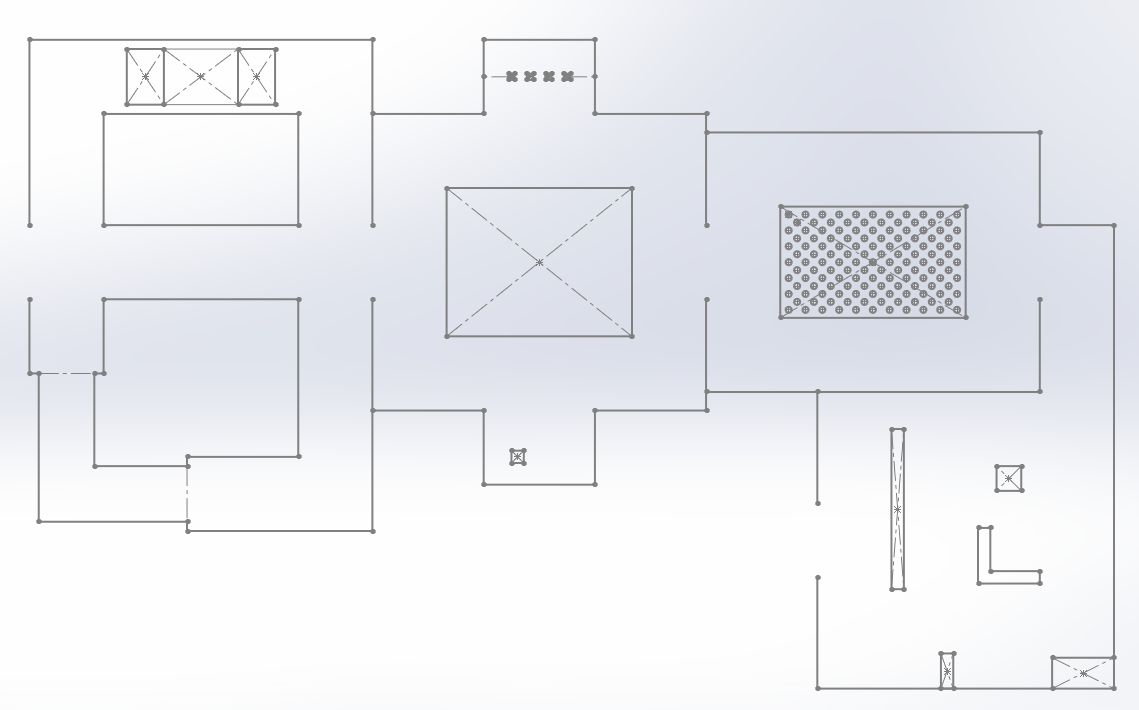
\includegraphics[scale=.5]{images/track_overview_wlabels.jpg}
	\caption{Field Overview}
	\label{fig:field} 
\end{figure}

\subsection{Track}
The Track is defined as a 24 inch wide path that is bounded on either side by 3 inch high walls. The walls used at the Competition will be constructed from foam board of the type that is easily obtainable from craft stores; 1/8 inch thick with a matte, white paper surface. The track floor will be short pile carpet.

\subsection{Rough Terrain}
The Rough Terrain section is a 3 feet wide by 5 feet long area covered with an array of domes aligned in a diagonal grid pattern. The domes are 3D printed plastic with a base diameter of 2 inches and a height of 1/2 inch. There will be walls on the long edges of the section, with bypass paths extending another 24 inches beyond the section walls. This Obstacles tests the durability and agility of the robot.

\subsection{Obstacles}
The 2020 Competition Track does include paths that bypass most Obstacles. Teams may choose to bypass any or all of the Obstacles during a run. See section \ref{bypass} for details.

\subsubsection{Tunnel}
The Tunnel is an L-shaped wooden structure with openings on either end that are 12 inches high by 18 inches wide. The interior is dark. This Obstacle tests the maneuverability of the robot in a confined space with limited visibility.

\subsubsection{Bridge}
The Bridge is 24 inches wide with a smooth wooden surface and no guard walls. The climb is 30 degrees with 12 inch rise, followed by a 24 inch span and a 30 degree descent. This Obstacle tests the robot’s ability to move in a controlled manner on an inclined surface.

\subsection{Object Identification and Handling}


\subsection{Obstacle Avoidance}
The Obstacle Avoidance section is defined as a 6 feet wide by 8 feet long rectangular area, as shown below. The Robot must navigate from the start to the finish without contacting walls or obstacles. Obstacles are defined as 2 inches deep by 4 inches high. There will be a maximum of 6 obstacles in the section. This section will be offered in 3 versions of varying autonomy.

\begin{itemize}
    \item Manual - Known Placement
    
        The Network will remain enabled and the Operator will have full control of the Robot as it navigates the section. If this option is chosen, the section will be laid out as defined below.
    \item Autonomous - Known Placement
    
        The Network will be disabled and the Operator will lose contact with the Robot. The Robot must be able to navigate the course autonomously. If this option is chosen, the section will be laid out as defined below.
    \item Autonomous - Unknown Placement
    
        The Network will be disabled and the Operator will lose contact with the Robot. The Robot must be able to navigate the course autonomously. If this option is chosen, the layout of obstacles in the section will be unknown to Teams until after the deadline to submit Robots on the day of the Competition. 
        
\end{itemize}
\section{The Game}
The order in which robots go through the track will be determined by lottery and may be reordered at the discretion of the event organizers. 
%The day will start with an organized practice run where teams will also be called upon to demonstrate their Loss-of-Signal handling (see section~\ref{los}). Due to a large number of teams that will need to practice each team will be restricted to a maximum of two members on the track during the practice runs.

\subsection{Objective}
The objective of the game this year is to navigate the entire track, which involves a variety of obstacles and prescribed tasks, letting the robot operate both autonomously and under operator control.

\subsection{Run Times}
Each team will be allowed a maximum of 20 minutes of operating time during the competition. The 20 minutes is divided into two sections: 5 minutes for setup and 15 minutes to run the track. The setup time ends when the robot begins operating. If the team uses more than 5 minutes for setup, it will cut into the 15 minutes of run time. 

The teams may attempt up to 3 runs within the 15 minute time window. At any time during the 15 minute run time, a team may choose to terminate the run and restart the track. A team may not restart after starting its third and final run. When the final run is started, it must be completed before the 15 minute window expires. A run in-progress will be terminated at the 15 minute mark, and the score for that run recorded at that time.

If a robot cannot complete the track in the allotted time, or if it runs out of time during a run, then “Did Not Finish” (DNF) is recorded along with the score for that run. A DNF score cannot be considered for the purpose of selecting a champion. Additionally, robots that obtain DNF scores will be ranked among themselves in a second, lower category. A DNF score will not be recorded for bypassing a section unless the robot is otherwise unable to complete the track.

If a robot is unable to start a run during the 20 minute operating period, it is recorded as “Did Not Start” (DNS).

In the event that the site communication link fails, the clock may be stopped or reset at the judges’ discretion.
\subsection{Scoring}
For the score of a particular run to be considered valid for the purpose of selecting a champion, the robot must perform a complete run of the track.

The score for each run is calculated using the following formula:

\[Score = (S_1 + S_2 + S_3(1-\frac{C_{S_3}}{5}) + S_4(1 - \frac{C_{S_4}}{5})) + T_b(1 - \frac{T_{r}}{T_{tot}}) - 50R\]

\ctable[caption=Scoring Variables, pos=h, label=tab:score] % options key=value,...
	{clll} % coldefs for \begin{tabular}
	{} % zero or more \tnote commands
	{ % table rows for the table
	\FL
		 				&						&   Values						    & Notes
	\ML
		$S_1 $ 			&	Bridge/Tunnel 		&	0,90,150 						& 150 if crosses bridge, 90 if takes tunnel, else 0 \\
		$S_2 $			& 	Object ID/Handling	& 	$0,100,200,300$			                    & Details below  \\
		$S_3 $          &   Rough Terrain       &   200                           & Maximum points for $S_3$ \\
		$S_4 $          &   Obstacle Avoidance  &   75,175,300                      & 75 if manual, 175 if autonomous (known) \\
		                &                       &                                   & \/ 300 if autonomous (unknown) \\
		$C_{S_3}$		&	Contact Penalty in $S_3$	& $0\leq C \leq 5$		& Times the robot touches the inner wall in $S_3$ \\
		$C_{S_4} $			&   Contact Penalty in $S_4$		&	$0 \leq C \leq 5$		 	    & Times the robot touches an obstacle in $S_4$\\
		$W $			& 	Wall Contacts 		& 	$0 \leq W$					    & Times the robot touches a wall\\
		$T_{r}$		    &	Run Time 	 		&	$0 \leq T_{r}+3W $  	& Run Time in seconds, including contact penalties \\
		$T_{tot}$	&	Total Time			& 	900				& Total available run time in seconds \\			
		$T_{b}$			& Time Bonus			&	300 				& Maximum time bonus \\
		$R $			& 	Reset Penalty 		&	$0 \leq R$					    & Number of times the handler touches robot
	\LL
	}
	
\subsubsection{Section 1 - Bridge/Tunnel}
If the robot crosses the bridge unaided, 150 points are awarded. If the robot successfully navigates the tunnel, 90 points are awarded. If the robot takes the bypass or is otherwise aided, 0 points are awarded.
%The variable $T$ is initially zero and increments by fifteen points for each of the first two times the robot makes contact with the Tunnel. Further impacts with the Tunnel do not result in $T$ increasing beyond 30, and do not count as Contact Penalties. 

\subsubsection{Section 2 - Object Identification and Handling}

Robots that identify and place the 10 Hz oscillator in the bright yellow bin will be awarded 300 points. 200 points are awarded for identifying and securing the 10 Hz oscillator. 100 points are awarded for securing any other cube. 100 points are awarded for placing any cube in the yellow bin. Only the first cube to be secured will be scored. 

\subsubsection{Section 3 - Rough Terrain}
A maximum of 200 points are available for completing the rough terrain section. 40 points are deducted for each contact with the inner walls of the section. Extended contacts may be recorded as multiple penalties at the judges' discretion. Completion is defined as the robot navigating from start to finish without more than half of the robot crossing the section boundaries.

$C_{S_3}$ represents the number of times the robot contacts the inner walls of the section.

\subsubsection{Section 4 - Obstacle Avoidance}
$S_4$ represents the maximum possible points available for the obstacle avoidance section. These maximums are as follows: 

\begin{itemize}
\item Manual - 75 points
\item Autonomous (Known placement of obstacles) - 175 points
\item Autonomous (Unknown placement of obstacles) - 300 points
\end{itemize}

$C_{S_4}$ represents the number of times the robot contacts obstacles in the section. Teams will be given 1 free contact, after which $C_{S_4}$ will increment by one per contact. Extended contacts may incur multiple penalties at the judges' discretion. Note that $C_{S_4}$ is not affected by contacts with course boundaries, which are defined in Section \ref{Wall Contact}.


\subsubsection{Time Bonus}
$T_b$ represents the maximum possible time bonus. To qualify for the time bonus, the robot must both finish the track and use no more than two bypass routes.

\subsection{Penalties}
\begin{itemize}
\item \textbf{Robot Reset} – If the robot handler has to touch the robot during the run it will result in a score penalty of 50 points and the robot will be put where it left the track or anywhere it has previously traveled. If any other team member touches the robot during the run, the current run will be disqualified and therefore not scored.
\item \textbf{Excessive Communication} – If the judge rules that any team member at the competition site is providing directions to the operator during a run, the team may be issued a warning, penalty or be disqualified depending on the extent of the infraction. The only communications recommended between the operator and the robot handler are “Start when ready” and “Terminate this run?” 
\item  \textbf{Wall Contact}\label{Wall Contact} – If the robot comes into contact with the track walls or crosses over track boundaries a penalty of 3 seconds will be added to the robot's run time. The penalty will be assessed each time the robot comes into contact with the boundaries. Extended contact can be assessed multiple penalties if it lasts longer than three seconds and the robot remains in motion. For example, a robot that stops while touching the boundary will only receive one penalty while one that drives while touching the wall might receive a series of penalties at the judge’s discretion.
\item \textbf{Bypassing an Obstacle}\label{bypass} -- There are bypass routes available for most sections. If a robot bypasses a section, the team will receive no points for that section. There will be no additional penalties assessed for bypassing the section. However, the robot may incur other penalties during the route.  
\end{itemize}

%\subsection{Scoring Examples}

%Robot 1 performs it’s final run flawlessly; it incurs no penalties, scores maximum points for the Delivery, and executes the Sprint in 10 seconds.
%
%\ctable[caption=Total Score for Robot 1, pos=h, label=tab:ex1] % options key=value,...
%	{ccccccccccc} % coldefs for \begin{tabular}
%	{} % zero or more \tnote commands
%	{ % table rows for the table
%	\FL
%	Score	&	P 	& 	T	&	 B   & 	S 	& $D_b$ 	& $D_m$ 	& $t_{sprint}$ 	& W 		& R 	& 	DNF
%	\ML
%	221     	&	30	& 	0	&	 30	& 	0 	& 25 	& 2 		& 10 			& 0 		& 0 	& 	False
%	\LL
%	}
%
%\newpage	
%Robot 2 successfully performs the Pickup, but scores no points in the Tunnel due to impacts. It is able to cross the Bridge on the third attempt; the first two attempts resulted in Robot Resets. Robot 2 is able to score Maximum points for the Delivery and sustains one contact penalty while negotiating the Slalom. The time allotted for Robot 2 runs out during the Sprint.
%
%\ctable[caption=Total Score for Robot 2, pos=h, label=tab:ex2] % options key=value,...
%	{ccccccccccc} % coldefs for \begin{tabular}
%	{} % zero or more \tnote commands
%	{ % table rows for the table
%	\FL
%	Score	&	P 	& 	T	&	 B   & 	S 	& $D_b$ 	& $D_m$ 	& $t_{sprint}$ 	& W 		& R 	& DNF
%	\ML
%	105     	&	30	& 	30	&	 30	& 	10 	& 25 	& 2 		& 50				& 1 		& 2 	& True
%	\LL
%	}
%
%Robot 3 is able to successfully perform the Pickup, but incurs a Contact Penalty while passing under the Bridge. It contacts the inside of the Tunnel once and is able to cross the Bridge on the first attempt. While getting into position to Deliver the Payload it makes two additional wall contacts. The robot places the circular Payload in the Delivery Zone. With less than a minute left, the team opts to take a Reset Penalty to bypass the Slalom. The Sprint is completed in 5 seconds.
%
%\ctable[caption=Total Score for Robot 3, pos=h, label=tab:ex3] % options key=value,...
%	{ccccccccccc} % coldefs for \begin{tabular}
%	{} % zero or more \tnote commands
%	{ % table rows for the table
%	\FL
%	Score	&	P 	& 	T	&	 B   & 	S 	& $D_b$ 	& $D_m$ 	& $t_{sprint}$ 	& W 		& R 	& DNF
%	\ML
%	95.375  	&	30	& 	15	&	 30 	& 	30 	& 15 	& 1		& 5				& 3 		& 1 	& False
%	\LL
%	}
	
%\subsubsection{Ranking Example}
%
%\ctable[caption= Example Ranking, pos=h, label=tab:rank] % options key=value,...
%	{lcr} % coldefs for \begin{tabular}
%	{} % zero or more \tnote commands
%	{ % table rows for the table
%	\FL
%	Rank			&		Robot Name 	&  	Score
%	\ML
%	Champion		&		Robot 1		&	221 \\
%	Second		&		Robot 3 		& 	95.375
%	\ML
%	Third		&		Robot 2		&	105
%	\LL
%	}
\section{The Robot}
\subsection{General Robot Requirements}
All work on the robot shall be completed by \textbf{8:30 AM \competition}, at which time all competing robots are to be turned off and put on display. Minor adjustments, such as the tightening of screws or the replacement of components that have fallen off, are permissible only during a team’s fifteen minute run time. Violation of this requirement will result in a warning, penalty, or disqualification at the judge's discretion.

\subsection{Safety}
We strongly encourage all teams to consider the safety of their fellow participants, the public and the venue when designing their robot. We reserve the right to disqualify any team whose robot is considered to fall short of safety standards. The following are required:

\begin{itemize}
\item Batteries: You may use NiCad, NiMH, SLA batteries or other "safe" batteries. Li-ion batteries may be used only if the team can demonstrate that proper charging and low voltage cut-off systems have been implemented. Low voltage cut-off systems must include a protection circuit that disconnects the battery from all Robot systems.
\item Switches: At minimum, Teams must implement two switches. The first must disconnect the batteries from all Robot systems. The second must disable the drive system. Both switches must be clearly identified in the technical documentation and easy to identify and reach on the Robot. 
\item Rocket motors, Medieval flails, Nuclear devices (that includes both fusion and fission) and any components that have a tendency to combust, explode, or jump-start the apocalypse are strictly prohibited.
\end{itemize}

\subsection{Communications}
The Competition provides an 802.11b/g/n Wi-Fi network on the venue. All communications between the driver and the robot must use this network. The driver must establish a two-way communication with the robot. At the very least, the robot must send a heartbeat signal back to the driver.

The following are the details of the wireless network and regulations of its use during the competition:

\begin{enumerate}
\item The Competition Wi-Fi network will have the ESSID “MERCURY” and \textit{no security protection}. This ESSID will not be broadcast. Please ensure that your system can connect to a Wi-Fi network without the ESSID broadcast.
\item The Wi-Fi router providing this network will have a public IP address that will be disclosed to the team on the day of the Competition.
\item Each team is allowed to have at most \textbf{three} networked hosts using the Wi-Fi network. For example, an IP camera and a Wi-Fi device will count as two hosts. A Wi-Fi device with a non-IP camera attached only counts as one host (for example, a smartphone providing video feed will only count as one host, but it must use the Wi-Fi network).
\item The team will have to provide information about their networked devices on the online registration form. The team may change this information on the form any number of times up until \textbf{\network}. This information includes a brief description of each device, the MAC addresses, and the ports each device will use if an inbound connection is required.
\item The networked devices will have to use DHCP to obtain an IP address. Static IP addresses are not allowed and will result in the team's disqualification if used. IP addresses are assigned based on the MAC addresses of the networked devices provided by the team on the registration form.
\item If the team requires an inbound connection to a networked device, the team is allowed to have at most three forwarded ports. The information provided on the registration form will be used and the team will be notified of the external ports assigned to the team a week before the competition.
\item During a team's run, only that team's robot and its associated devices will have access to the Wi-Fi network. \textbf{\textit{All other robots and devices that access the Competition router must be completely turned off.}} Failure to do so will result in the team being issued a warning, a penalty or disqualified.
\item A base station to provide non-Wi-Fi wireless link between the robot and the official router is allowed to be used on-site. This wireless link must not use the 802.11 standard. The base station must use the competition Wi-Fi network to gain Internet access and the base station will count towards the three maximum networked devices.
\item Independent Wi-Fi repeaters, bridges, ad-hoc Wi-Fi networks, and access points are not allowed. The only 802.11b/g network each device may use is the official wireless network.
\CT{\item If the team chooses to attempt an autonomous version of the Obstacle Avoidance section, the network will be disabled when the Robot reaches the beginning of that section. The Robot is still required to indicate a loss-of-signal event. The indicator must be described in the technical documentation such that competition judges can easily identify the state of the Robot's wireless connection. If the Robot continues through the Obstacle Avoidance section without indicating a loss-of-signal event, it will be scored as if it is controlled manually.}
\end{enumerate}

\subsubsection{Loss-of-Signal Test}
\label{los}
The team must pass a “Loss-of-Signal” (LOS) test to be eligible as the Competition champion. Teams will have two opportunities to demonstrate LOS handling: \textbf{\los} during the evening Practice period and during regular testing the morning of \textbf{\competition}.

The test will be performed as follows:

\begin{enumerate}
\item The team clearly demonstrates that the driver can control the robot,
\item The official router technician will then shut down the router and the robot must be able to clearly indicate that it is now experiencing a loss-of-signal situation and stop,
\item After the official router is restarted, the team must be able to demonstrate that the driver can re-establish connection to the robot without the team personnel manipulating the robot. The robot must show that connection is re-established by turning off the Loss-of-Signal indicator, and resume normal operation as in point 1.
\end{enumerate}
\section{The Tournament}
\subsection{Registration}
Registration forms can be found online at \url{http://mercury.okstate.edu} under the Mercury Challenge tab. Registration information should be submitted no later than \textbf{\registration}. The registration forms provide information that is needed to organize the competition, generate name tags, and for preparing refreshments. Please contact us if you have special dietary needs.

The competition is open to teams of any size though only four members may hold active positions at the competition. The active positions and their responsibilities are:

\begin{itemize}
\item Team Leader – The team leader is the contact point between the competition organizers and the team. The team leader is encouraged to be at the venue or to have a representative standing in during the day of the competition and may act as the robot handler or a technical assistant.
\item Operator – During the competition only the Operator may guide the robot. Note that, unlike previous years, the Operator is no longer required to be 50 miles (80km) away from the competition site. There will be a room provided at the competition venue for the Operator to guide the Robot. If the Operator is located on the OSU campus, he or she must control the Robot from the provided room. There is no other restriction on the location of the Operator.
\item Robot Handler – During the competition only the Robot Handler may touch the robot during a run. Permitted contact includes any technical support or maintenance.
\item Technical Assistant – During the competition the technical assistant may only handle the robot whenever a “run” is not in progress. The technical assistant is to provide aid with technical issues that may arise with the robot.
\end{itemize}

Teams are encouraged to come up with a unique team name that will be used for keeping score and for announcements at the competition. 

\subsection{Practice Runs}
Track setup will begin \textbf{\los \ at 5 pm} at the Competition venue. During the setup period teams will be allowed to test their robots on the Track as it is being assembled. The Competition router will also be available for testing. Additionally, robots can undergo LOS testing at this time. Teams are encouraged to contact us ahead of time so that staff is available to assist them when they arrive.

\subsection{Documentation}
In order to participate in the competition, each team is required to provide a documentation package that is to be submitted via email to \href{mailto:okstate.mercury.robotics@gmail.com}{ okstate.mercury.robotics@gmail.com} no later than \textbf{\documentation}. This section describes all submission items that comprise the documentation package.

\subsubsection{Technical Document}
The technical document describes the robot and the design decisions that go into the robot. There is a 10 page limit to this document NOT including appendices. This document will be used by the competition officials to survey the technology and engineering methods used by the team to improve subsequent competitions. 

At the minimum, please ensure that the document addresses the following topics:

\begin{itemize}
\item A high-level block diagram of the robot including both electrical (batteries, sensors, relays, etc.) and mechanical systems (drive train, motors, belts, gears, etc.)
\item Safety systems (battery protection (fuses, protection circuit), kill switch, etc.)
\item Communication systems used (TCP or UDP sockets, applications, etc.)
\item The main controller used for the robot (single-board computers, Arduino, custom made, etc.)
\item Video feedback system (if the robot has it)
\item The driver interface of the robot
\item Parts list/Bill of materials
\item A general description of any autonomous and logical subsystems
\item Power subsystem	
\end{itemize}
This document is a factor for the “Best Design” award. Please submit this document in PDF format.
\subsubsection{Video Presentation}
Each team is required to submit a 2 to 5 minute video for the competition. This video will be used for promotional materials for the competition and will be played during the competition itself for the audience, so please tailor the contents of the video accordingly and ensure that the robot is actually featured! The video is a factor for the “Best Presentation” award. Please upload your team’s video to a video hosting service, preferably YouTube or Vimeo, and include a link to it with your documentation package submission. While videos may be humorous, please refrain from including profanity of any kind. Videos found to contain profanity will be disqualified from the ``Best Design'' award and will not be featured on the Mercury web page.

\subsubsection{Robot and Team Picture}
Teams are required to submit a reasonably high-resolution picture of the robot (300 dpi) and a picture of the team personnel. These pictures will be featured in promotional materials and miscellaneous items in the competition such as team member badges, posters, displays, etc. The picture must be in JPEG or PNG format. Please submit the picture with your documentation package submission.

\subsection{Judging}
A panel of OSU Mercury Robotics officers and OSU professors will be responsible for judging the performance of the robot during the competition (penalties, starting time, etc.). The judges will also be in charge of scoring the video presentation, the robot design, and interviewing participants to determine the winners for Judges’ Choice awards. 
Any subject not considered in this document will be left to the discretion of the judges.

\subsection{Awards}
The awards will be given to the three highest scores computed during the competition, resulting in the 1st, 2nd, and 3rd place respectively. Other Awards will include: “Best Presentation” (submitted video presentation), “Best Design,” and “Judge's Choice.” Note that it is possible for one team to win multiple awards. 
Awards, except the ones based on the team’s score, will be given at the discretion of the Judges. They may base awards on personal preference or by examining the general consensus of teams, volunteers, and spectators. 
\section{Appendix}
\subsection{Important Dates}
\textbf{Please note that the cutoff time for each deadline below is 11:59:59 PM CST.} \\

\begin{tabular}{ll}
Registration Deadline					&	\registration		\\
Documentation Submission Deadline		&	\documentation	\\
Deadline to Update Network Information	&	\network			\\
									&	\\
Practice, Early LOS Testing				&	\los 			\\
Competition							&	\competition 		\\

\end{tabular}

\subsection{Contact Information}
If you have any questions regarding the information in this document or in relation to the Competition, visit our website at \url{http://mercury.okstate.edu} or contact us via email at \href{mailto:okstate.mercury.robotics@gmail.com}{ okstate.mercury.robotics@gmail.com}.

\vfill
\begin{center}
{\huge We look forward to seeing you at the 2019 Mercury Remote Robot Challenge}
\end{center}

\end{document}